\section{Feedback}

\subsection{Listing Mistakes}
\label{sec:feedback-listing}
\todo[inline,color=red]{Feedback Techniques - List of Issues}

- Very clear what's wrong

- Comes across negative

- Doesn't necessarily help them know what to do next time

- Easy to generate

- Didn't always mean much to the child

\subsection{Colour Coding}
\todo[inline,color=red]{Feedback Techniques - List of Issues}

- Nice and visual

- Can highlight component by component (perhaps in conjunction with \cref{sec:feedback-listing}

- Traffic Light system

- Didn't always mean much to the child

\subsection{On Screen Correction}

- Scaling, Rotation, Translation

- Animations were very clear :)

- Hard to do! Lots of potential difficulties

- Child immediately got what they'd done wrong

\subsection{Aggregation}
Given the large number of scoring results given for a manuscript drawing, some of the early testers suggested that a simple scoring system could be used like stars from 1 to 3 or 1 to 5.

To produce a simple numeric score we must somehow aggregate the more detailed feedback. For example, by assigning weights to `musical correctness', `stems', `note heads' etc, we can produce a score in a reasonable range for overall feedback in a more simplistic form.

\begin{figure}[H]
  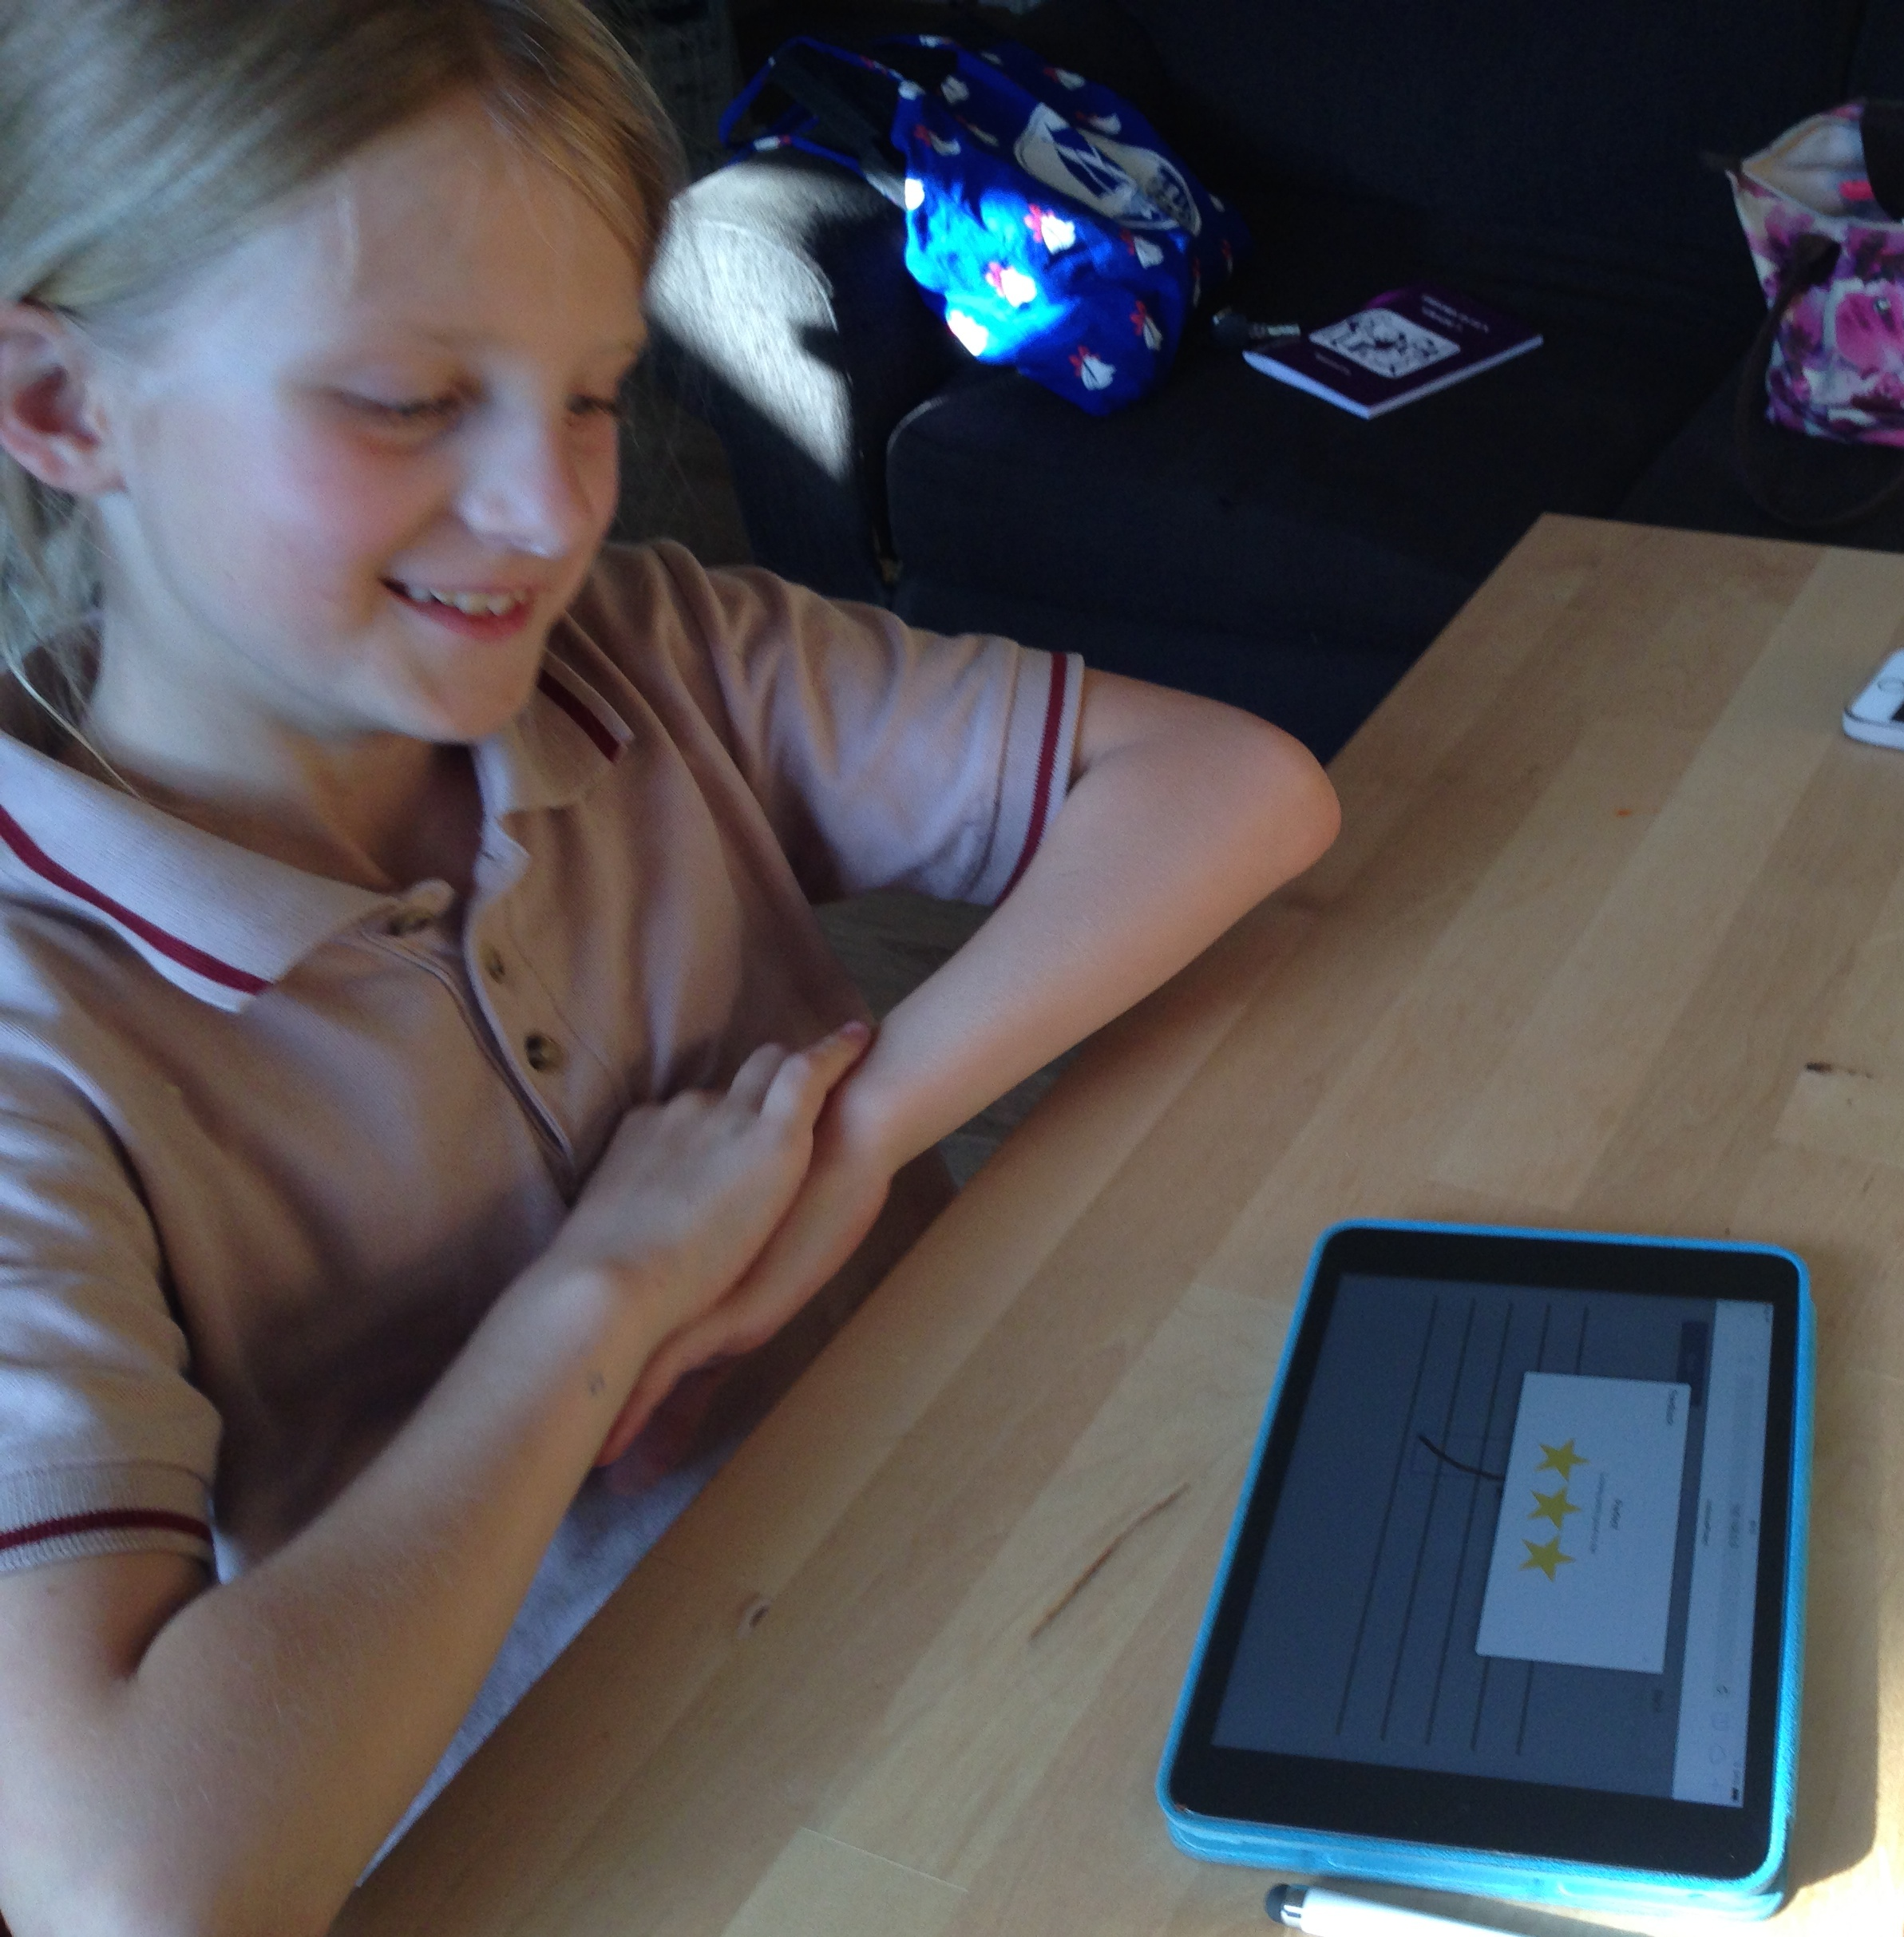
\includegraphics[width=\linewidth]{gfx/photos/user-receiving-feedback.jpg}
  \caption{Child receiving simplified graphical feedback}
\end{figure}
